\chapter{Producto. Análisis Teórico-Computacional}\label{chapter:proposal}

HCVet es una App móvil para gestionar y administrar historias clínicas de mascotas, donde los usuarios pueden tener registros de cada consulta que se ha hecho ,saber sus padecimientos y antecedentes de forma rápida y precisa. Esto es de mucha ayuda a la hora de atenderlas en las visitas al veterinario,y también para tener conciencia de los cuidados y la atención que se le debe dar.

Se tiene una Application Programming Interface(API) para manejar la sincronización entre los clientes, el producto al que se refiere esta tesis es precisamente a la API. La primera vez que una persona va a usar la app debe registrarse, por tanto debe conectarse al servidor, este le asignará dos espacios para registrar dos mascotas, en caso de querer más deberá realizar una suscripción.

La App cuenta con varias vistas para distintos tipos de consulta que se pueda hacer su mascota como patología, radiología, una visita médica regular, una cirugía, etc. Cada una cuenta con una serie de datos que se pedirán para llenar según el tipo de consulta. Los usuarios también podrán asignar a otros como \textbf{encargados} de sus mascotas, para que estos también puedan registrar consultas sobre  las mascotas de otros dueños, por ejemplo un familiar o amigo.

Una de las cosas más particulares que tiene este software es que está pensado para que casi todas sus funcionalides se pueden hacer fuera de línea (offline), o sea, sin estar conectado a internet. Se pensó de esta forma para evitar la total dependencia de un servidor, ya que a algunas personas les puede ser un poco difícil el acceso a la red. Debido a esto se tuvieron que hacer algunas modificaciones en la estructura del proyecto, para que el servidor pudiera hacer un proceso de sincronización, correcto y eficiente.Los datos de todos los usuarios estarán en el servidor, pero además cada uno tendrá sus datos particulares en una base de datos local en su móvil. 

\section{Casos de Uso}

La primera acción de un usuario es el registro de su cuenta. Para llevar a cabo esta acción es obligatoria una conexión a internet, de esta forma se puede validar en el registro en el servidor. Esta validación incluye verificar el nivel de seguridad de la contraseña y que el número de teléfono actual no esté ya registrado en el sistema. En la figura \ref{fig:signup_view} podemos ver los datos necesarios para el registro.
\begin{figure}[H]
	\centering
	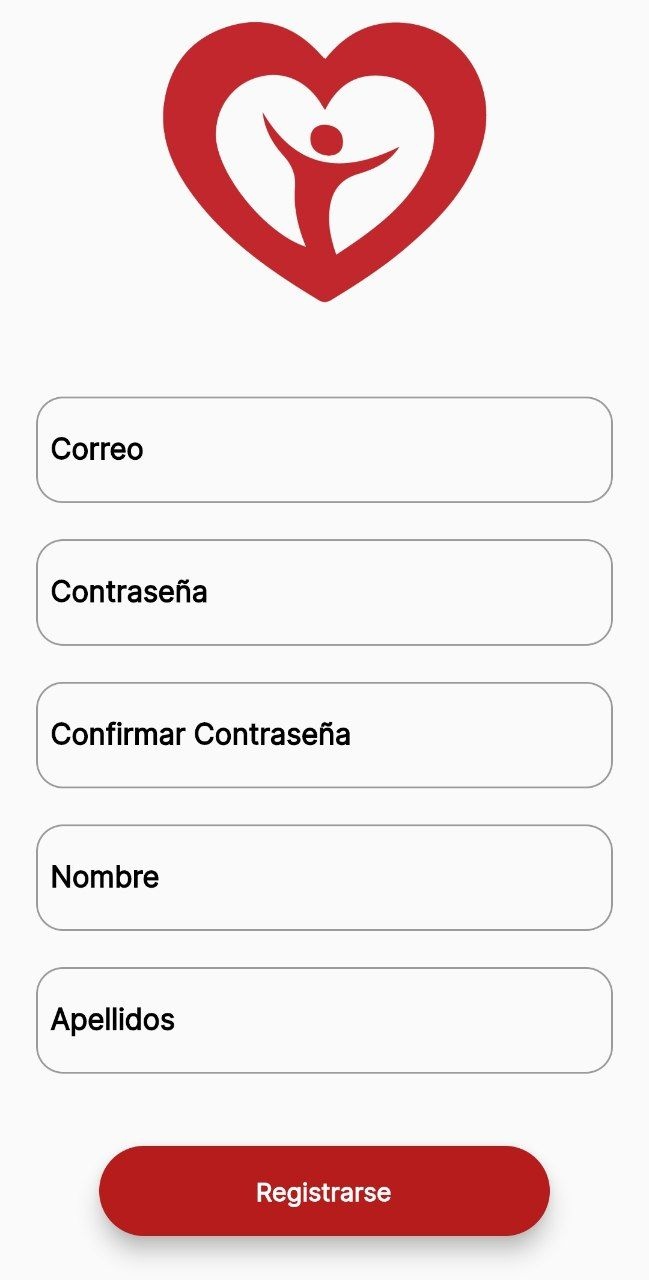
\includegraphics[width=7cm, height=10cm]{Graphics/signup_view.jpg}
	\caption{Vista para registro de usuario.}
	\label{fig:signup_view}
\end{figure}
Una vez que el usuario tiene una cuenta puede autenticarse a través de la vista que se ve en la figura \ref{fig:auth_view}. Desde el servidor se le asignará un token, el cual debe estar incluido en el encabezado de todas las peticiones http posteriores para verificar la autorización de acceso a los endpoints de la API.
\begin{figure}[H]
	\centering
	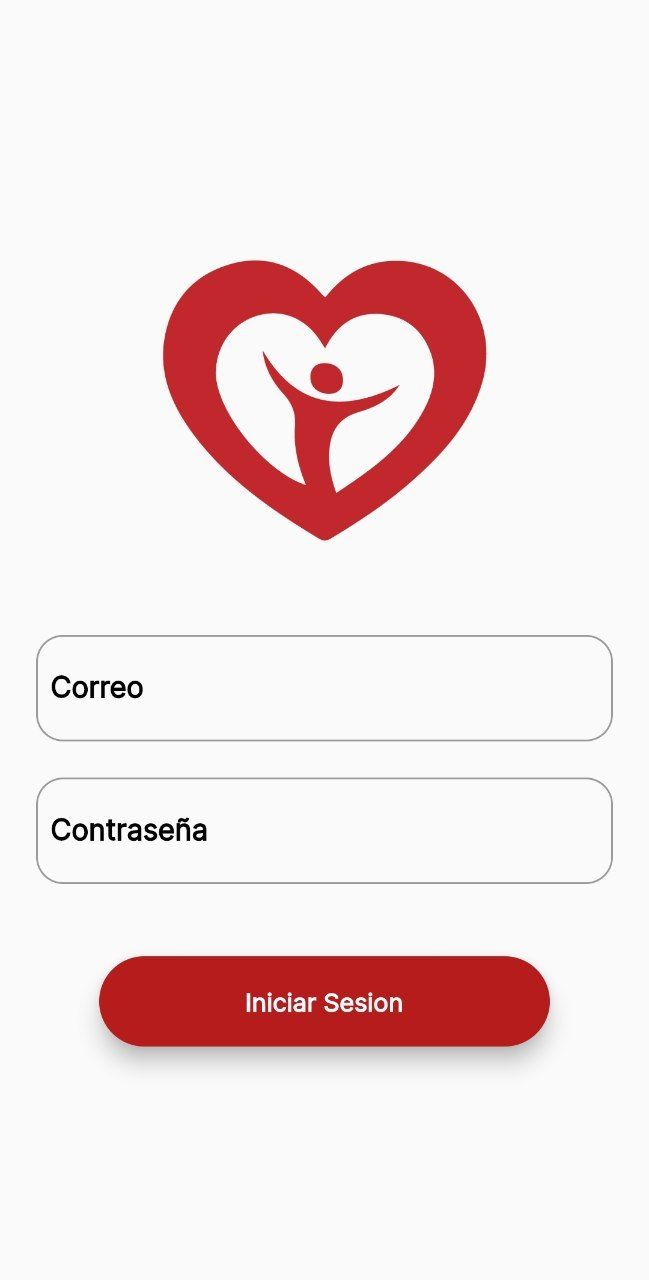
\includegraphics[width=7cm, height=10cm]{Graphics/auth_view.jpg}
	\caption{Vista para autenticación de usuario.}
	\label{fig:auth_view}
\end{figure}

La tarea más importante de la API, es la de sincronizar los datos de los usuarios para que la información se mantenga fiable y consistentemente. Este proceso de sincronización cuenta con las siguientes funcionalidades o casos de uso, que sí requieren de conexión a internet :
\begin{itemize}
	\item Subir datos al servidor :
	
	Los nuevos datos generados se subirán al servidor. Esto se realizó para tener una centralización de los datos, y de alguna forma una copia de seguridad de los mismos, en caso de pérdida. También sirve para el proceso de sincronización en usuarios que tengan mascotas en común, al tener esos datos en el servidor, proveerá esos datos a los usuarios que le sean requeridos.
	
	\item Bajar datos del Servidor :
	
	Todos los datos que hayan sido subidos al servidor, de todas las mascotas que el usuario sea dueño serán agregados a la base de datos local. Está función mantiene actualizados los datos de cada usuario, por ahora solo agrega datos, en un futuro se pudiera mejorar esta acción para que también actualice y elimine datos, que este proceso puede ser bastante complejo. 
	
	\item Asignar encargado :
	
	Se le notificará al servidor que un usuario ha sido asignado como encargado de una nueva mascota. Esta función es necesaria, para que el servidor pueda proveer de los nuevos registros tanto a los dueños como a los encargados.
	
		\item Desasignar encargado :
	
	Se le notificará al servidor que un usuario ha dejado de ser  encargado de una mascota. A la vez que un cliente deje de tener relación con la mascota, se deberá tener en cuenta para que no lleguen datos innecesarios a la hora de sincronizar   
\end{itemize}
Usualmente las actualizaciones son eventos que se ejecutan en la app cuando esta detecta que tiene conexión con el servidor. Pero existen en algunas vistas la posibilidad de solicitar una sincronización manual. En la figura \ref{fig:pets_view} se puede observar el botón de sincronización manual en la esquina superior izquierda.
\begin{figure}[H]
	\centering
	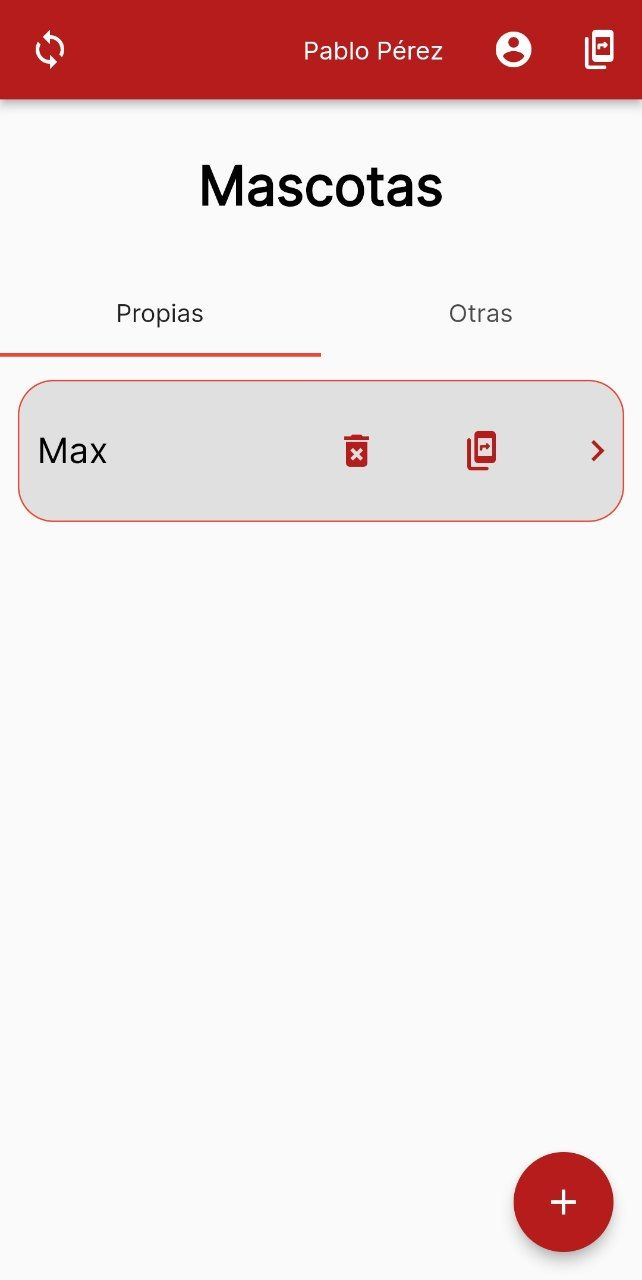
\includegraphics[width=7cm, height=10cm]{Graphics/pets_view.jpg}
	\caption{Sincronización manual.}
	\label{fig:pets_view}
\end{figure}

  \section{Propuesta de Arquitectura}
  
  Se tuvieron en cuenta varias arquitecturas, todas varían un poco en sus detalles, pero son bastante parecidas, ya que tienen un objetivo en común, la separación de obligaciones dividiendo el software en capas. Valorando la capacidad de extender la solución así como la testeabilidad de la misma en un futuro.
  
  \subsection{Clean Architecture}
  Clean Architecture ,popularizada por Robert Cecil Martin, es una arquitectura de capas, y
  en estas arquitecturas las capas se colocan de forma horizontal, donde una capa solo puede depender
  de otra que esté por debajo de ella, nunca por encima. Puede ver la figura \ref{fig:clean_architecture} que muestra a través
  de un diagrama la estructura y el flujo de esta arquitectura de forma general.\brackcite{cleanArchitecture}
  
\begin{figure}[!h]
	\centering
	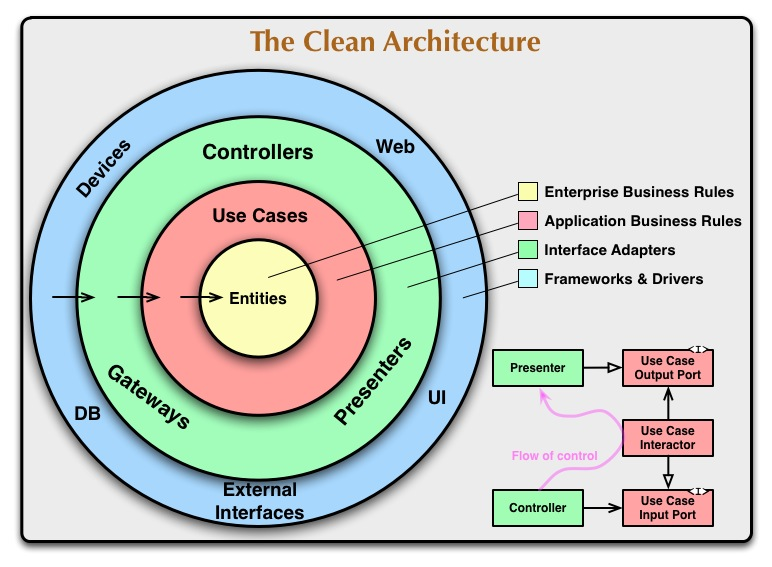
\includegraphics[width = 14cm]{MainMatter/CleanArchitecture.jpg}
	\caption{Diagrama de Clean Architecture }
	\label{fig:clean_architecture}
	
\end{figure}	

\subsubsection{Regla de dependencia}
  
  Los círculos concéntricos representan diferentes áreas de software. En general, cuanto más avance, mayor será el nivel del software. Los círculos exteriores son mecanismos. Los círculos internos son políticas.
  
La regla primordial que hace que esta arquitectura funcione es la regla de dependencia. Esta regla dice que las dependencias del código fuente solo pueden apuntar hacia adentro. Nada en un círculo interior puede saber absolutamente nada sobre algo en un círculo exterior. En particular, el nombre de algo declarado en un círculo exterior no debe ser mencionado por el código en un círculo interior. Eso incluye, funciones, clases. variables, o cualquier otra entidad de software nombrada.


Del mismo modo, los formatos de datos utilizados en un círculo exterior no deberían ser utilizados por un círculo interior, especialmente si esos formatos son generados por un marco en un círculo exterior. No queremos que nada en un círculo exterior impacte en los círculos interiores. \brackcite{cleanArchitecture}



\subsubsection{Uso de Arquitectura}
Para la implementación de esta arquitectura la aplicación se dividirá en las 3 capas descritas a continuación:

\begin{itemize}
	\item \textbf{Core}: La capa más interna, no es susceptible a cambios en otras capas, es totalmente independiente. Esta contiene la lógica de negocio, los objetos de uso general en la aplicación(entidades),el mapeo de las entidades, definición de interfaces a implementar tanto en esta capa como en las que la envuelven.
	
	\item \textbf{Infrastructure}: : La capa referente a datos, contiene las funciones correspondientes al acceso a base de datos(BD). Se subordina a las peticiones de la capa de dominio por medio de los
	Repositorios que implementan cómo acceder a los datos.Contiene los servicios y repositorios para proveer datos a las capas más externas.
	
	\item \textbf{API}: Expone los end-points de la aplicación, que son las funcionalidades explicadas anteriormente, esta es la capa más externa. Aquí se convierten los datos  en la forma más conveniente para cualquier marco de persistencia que se esté utilizando. Ningún código dentro de este círculo debería saber nada sobre la BD.
	
\end{itemize}
\newpage

\subsection{Modelo de Datos }

Para mantener una correcta sincronización entre todos los usuarios y tener una persistencia de  los datos es necesario el empleo de una base de datos(BD). Ahora bien, como se dijo aneriormente cada cliente tendrá una base de datos local en su móvil con los datos necesarios para satisfacer todas las consultas relacionadas con él,en cambio la BD de la API tendrá los datos de todos los usuarios. 

Primeramente se pensó un modelo teniendo en cuenta el buen diseño de una BD, cumpliendo con las normas y buenas prácticas para la ampliación del mismo de manera sencilla. Después de hacer un análisis se llegó a la conclusión de que las únicas operaciones de modificación de la BD de la API son crear  usuarios y mascotas, entonces se decidió diseñar un modelo totalmente dependiente de estas dos entidades que no es el ideal, pero es bastante bueno y garantiza una coordinación correcta en los datos. También se tienen unas tablas para guardar datos estáticos que son medicamentos, vacunas, enfermedades y alergias. Estas tablas serán persistentes en las BD de todos los dispositivos y no podrán ser modificadas. En la figura \ref{fig:model} se tiene una visualización del modelo.

\begin{figure}
	\centering
	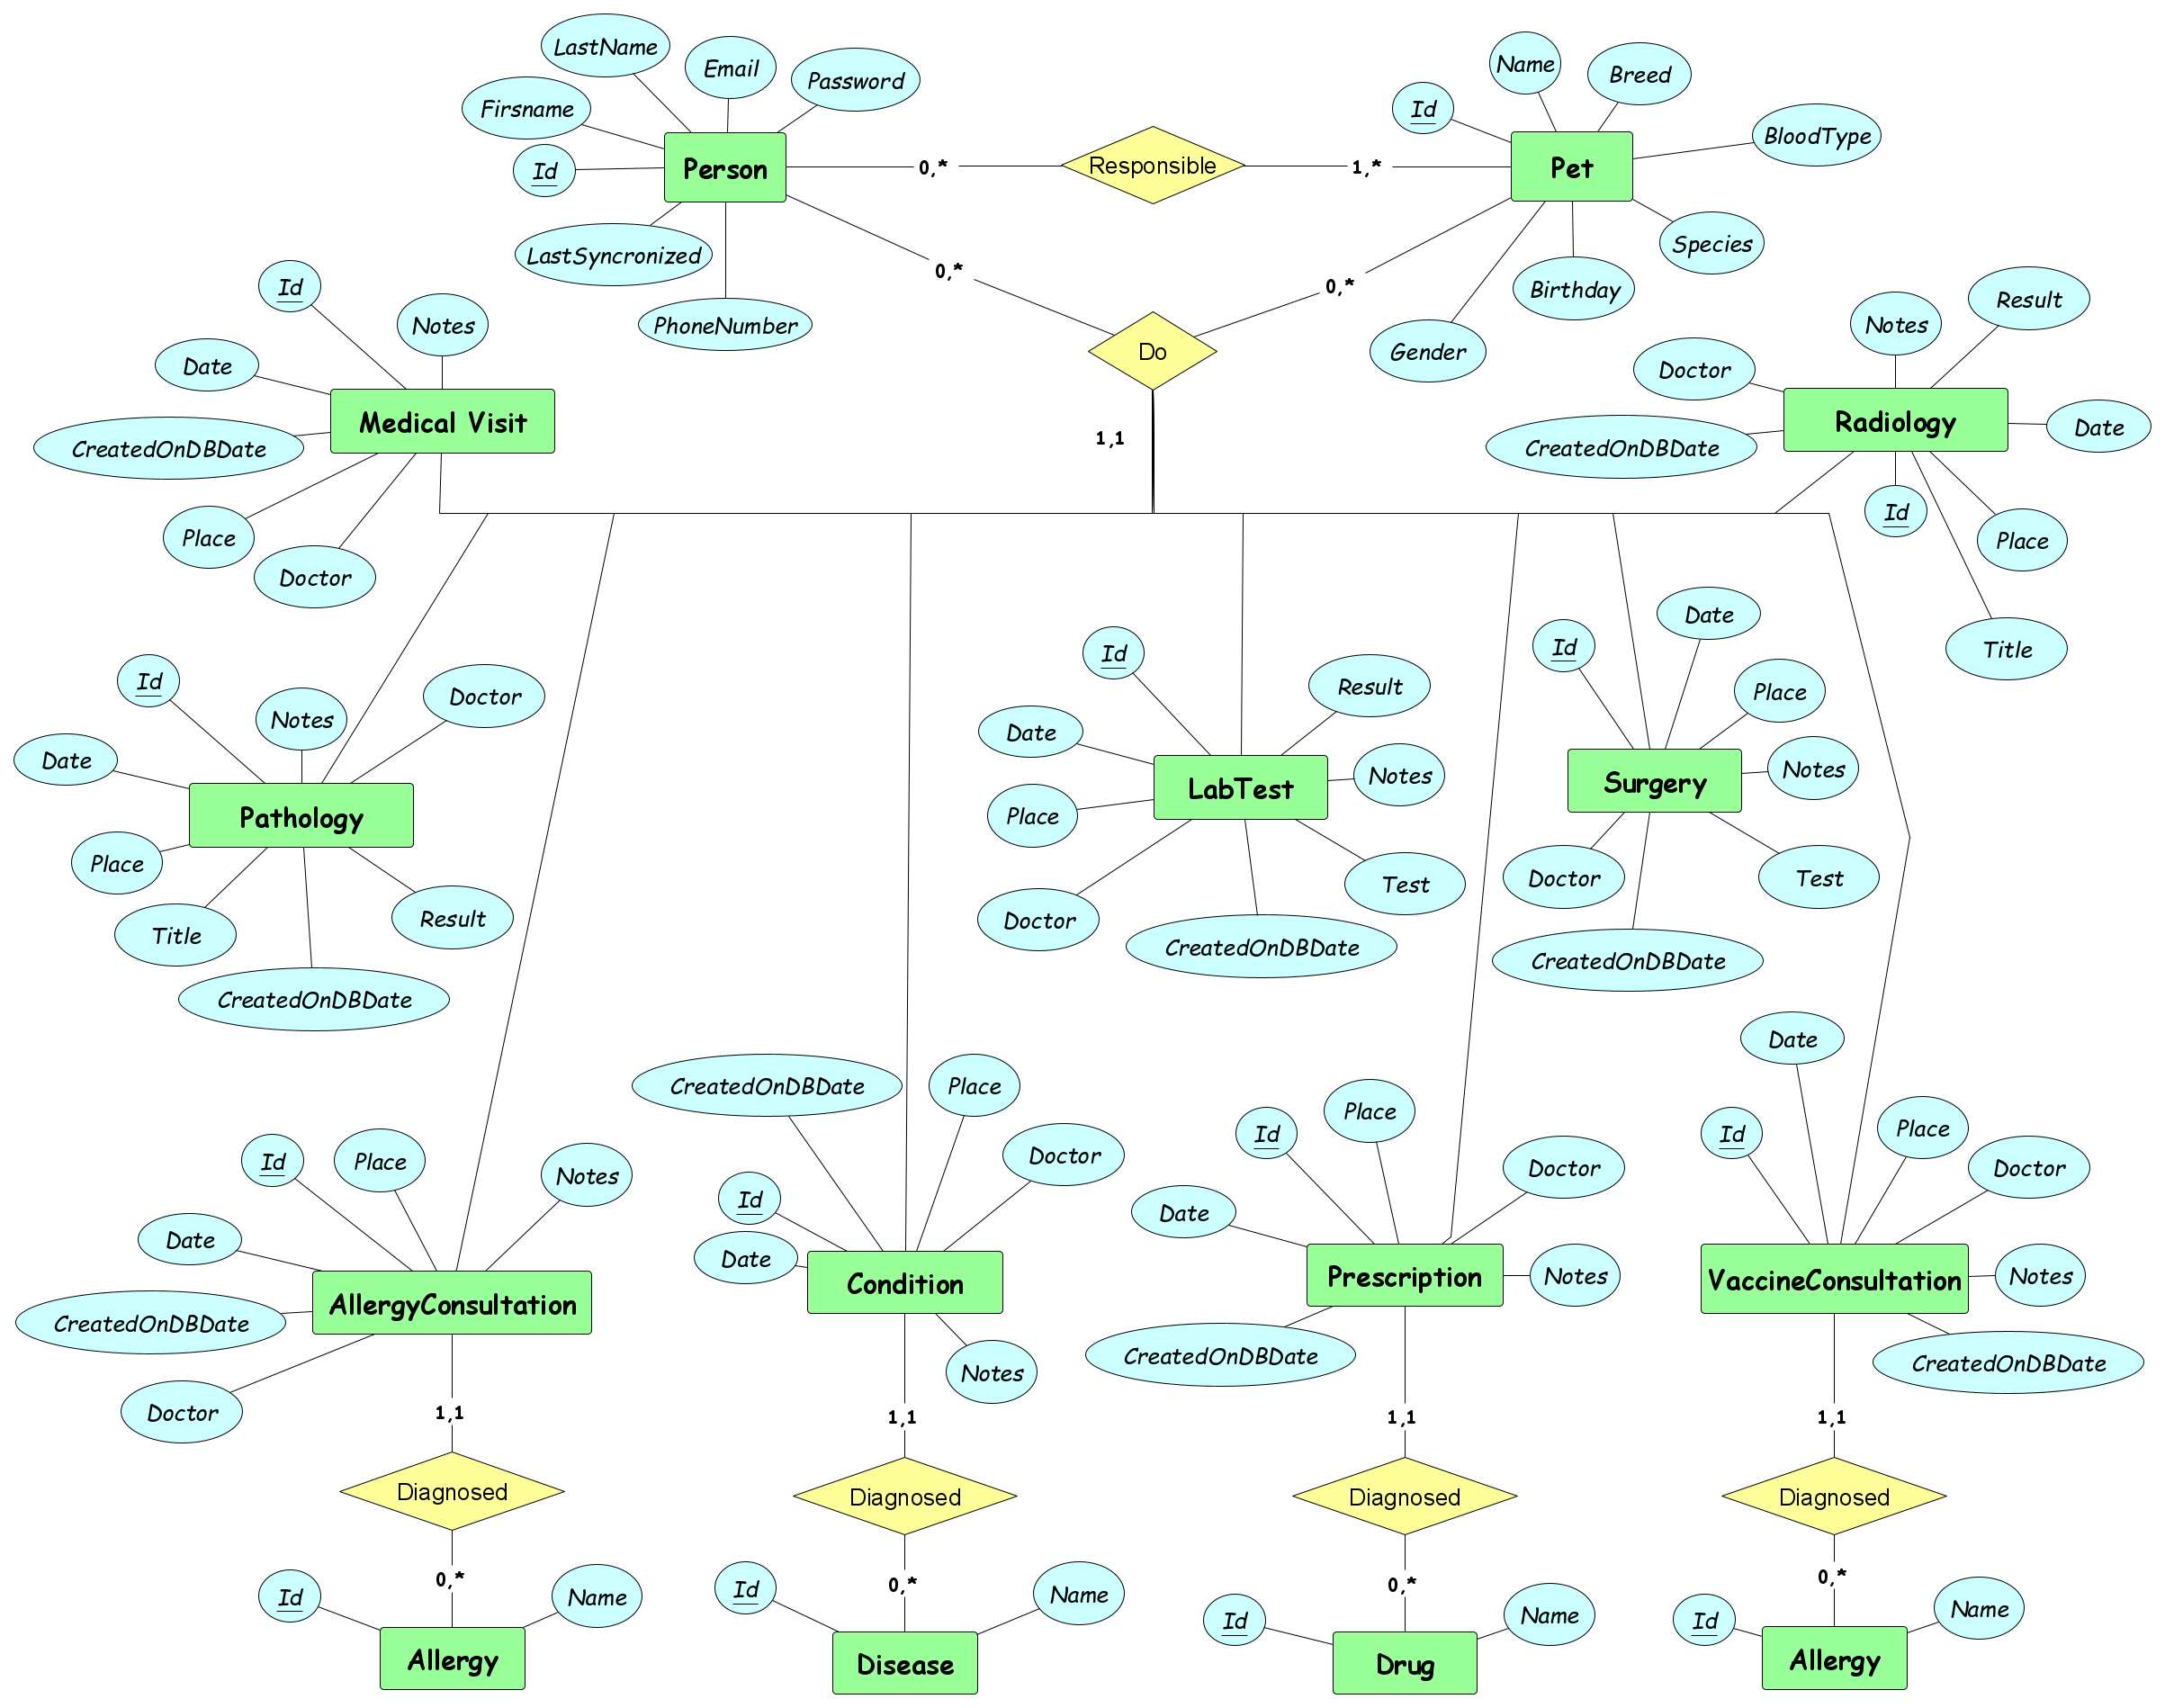
\includegraphics[width = 15cm]{MainMatter/model.png}
	\caption{Diagrama del Modelo Entidad Relacional }
	\label{fig:model}
	
\end{figure}	
\newpage

El modelo diseñado consta de \textbf{quince entidades} las cuales son descritas a continuación:
\newline


\textbf{User} es la tabla que contiene la información  de los usuarios, tiene más campos que hereda de Identity framework para cuestiones de seguridad, pero aqui solo se mostraran los necesarios para describir el modelo visto en la  fig \ref{fig:model}

\begin{itemize}
	\item	$Id$ ($PK$): Texto que identifica de forma única a un usuario.
	\item	$FirstName$: Texto utilizado para almacenar el nombre del usuario.
	\item	$LastName$: Texto utilizado para almacenar el apellido del usuario.

	\item	$Email$: Texto utilizado para almacenar la dirección de correo del usuario.
	\item	$Password$: Texto utilizado para almacenar la contraseña del usuario
	\item	$PhoneNumber$: Entero utilizado para almacenar el número de teléfono del usuario.
	\item	$LastSyncronized$: Fecha que almacena la última vez que el usuario se sincronizó con la bd, este dato juega un papel fundamental en la sincronización.
	
	
\end{itemize}


\textbf{Pets} es la tabla que contiene la información básica de las mascotas:

\begin{itemize}
	\item	$Id$ ($PK$): Valor entero que identifica de forma única una fila de esta tabla y por ende a una mascota.
	\item	$IdPerson$  ($FK$\footnote{Llave foránea, $Foreign$ $Key$ por sus siglas en inglés.} ): Texto utilizado para identificar de forma única al dueño de la mascota.
	\item	$Name$: Texto utilizado para almacenar el nombre de una mascota.
	\item	$Birthdate$: Texto utilizado para almacenar la fecha de nacimiento de una mascota.
	\item	$Species$: Texto que contiene la especie a la que pertenece una mascota.
	\item	$Breed$: Texto que contiene la raza a la que pertenece una mascota.
	\item	$Gender$: Texto que contiene el género de una mascota.
	\item	$BloodType$: Texto que representa el tipo de sangre de una mascota.
	
\end{itemize}

\textbf{Allergies}, \textbf{Drug}, \textbf{Vaccines} y \textbf{Disease} son las tablas que contienen las definiciones por defecto de las alergias, los medicamentos, las vacunas y las enfermedades respectivamente:

\begin{itemize}
	\item	$Id$ ($PK$\footnote{Llave primaria, $Primary$  $Key$ por sus siglas en inglés.} ): Valor entero que identifica de forma única cada una de las filas de estas tablas.
	\item	$Name$: Texto utilizado para nombrar una alergia, un medicamento, una vacuna o una enfermedad dependiendo del caso.
	
\end{itemize}

\textbf{MedicalVisit} es la tabla que contiene la información de las visitas médicas:

\begin{itemize}
	\item	$Id$ ($PK$): Texto que identifica de forma única una fila de esta tabla.
	\item	$IdPet$ ($FK$): Valor entero que identifica de forma única una fila de la tabla $Pets$.
	\item	$IdPerson$($FK$): Texto que identifica de forma única a la persona que insertó una visita médica en la aplicación.
	\item	$Date$: Texto utilizado para almacenar la fecha de una visita médica.
	\item	$Place$: Texto que representa el lugar en el que se realizó una visita médica.
	\item	$Doctor$: Texto que contiene el nombre del médico o especialista que realizó una visita médica.
	\item	$Notes$: Texto utilizado para almacenar notas extras sobre una visita médica.
	\item	$CreateOnDb$ 
	Fecha para identificar cuando fue generado este dato en la BD
\end{itemize}

\textbf{LabTests} es la tabla que se utiliza para almacenar las pruebas de laboratorio:

\begin{itemize}
	\item	$Id$ ($PK$): Texto que identifica de forma única una fila de esta tabla.
	\item	$IdPet$ ($FK$): Valor entero que identifica de forma única una fila de la tabla $Pets$.
	\item	$IdPerson$: Texto que identifica de forma única a la persona que insertó una prueba de laboratorio en la aplicación.
	\item	$Date$: Texto utilizado para almacenar la fecha en la que se realizó una prueba de laboratorio.
	\item	$Place$: Texto en el que se guarda el lugar en el cual se realizó una prueba de laboratorio.
	\item	$Doctor$: Texto que almacena el nombre del especialista que realizó una prueba de laboratorio.
	\item	$Test$: Texto que identifica el test realizado en una prueba de laboratorio.
	\item	$Result$: Texto que almacena el resultado de una prueba de laboratorio.
	\item	$Normal$ : Valor entero que representa si una prueba de laboratorio fue normal o no.
	\item	$Notes$: Texto utilizado para almacenar notas extras sobre una prueba de laboratorio.
	\item	$CreateOnDb$ 
Fecha para identificar cuando fue generado este dato en la BD
\end{itemize}

\textbf{Prescription} es la tabla que almacena las prescripciones:

\begin{itemize}
	\item	$Id$ ($PK$): Texto que identifica de forma única una fila de esta tabla.
	\item	$IdPet$ ($FK$): Valor entero que identifica de forma única una fila de la tabla $Pets$.
	\item	$IdMedicament$ ($FK$): Valor entero que identifica de forma única una fila de la tabla $Drug$.
	\item	$IdPerson$: Texto que identifica de forma única a la persona que insertó una prescripción en la aplicación.
	\item	$Dose$: Texto que representa la dosis del medicamento recetado en una prescripción.
	\item	$Date$: Texto que almacena la fecha en la que se realizó una prescripción.
	\item	$Place$: Texto que representa el lugar donde se realizó una prescripción.
	\item	$Doctor$: Texto que contiene el nombre del especialista que realizó una prescripción.
	\item	$Notes$: Texto utilizado para almacenar notas extras sobre una prescripción.
		\item	$CreateOnDb$ 
	Fecha para identificar cuando fue generado este dato en la BD
	
\end{itemize}

\textbf{AllergyConsultation} es la tabla que almacena las alergias de las mascotas.
\begin{itemize}
	
	
	\item	$Id$ ($PK$): Texto que identifica de forma única una fila de esta tabla.
	\item	$IdPet$ ($FK$): Valor entero que identifica de forma única una fila de la tabla $Pets$.
	\item	$IdAllergy$ ($FK$): Valor entero que identifica de forma única una fila de la tabla $Allergies$.
	\item	$IdPerson$: Texto que identifica de forma única a la persona que insertó una alergia en la aplicación.
	\item	$Date$: Texto utilizado para almacenar la fecha en la que se detectó una alergia.
	\item	$Notes$: Texto utilizado para almacenar notas extras sobre la detección de una alergia.
	\item	$CreateOnDb$ 
Fecha para identificar cuando fue generado este dato en la BD
\end{itemize}


\textbf{Condition} es la tabla para almacenar las condiciones o enfermedades que tienen las mascotas:

\begin{itemize}
	\item	$Id$ ($PK$): Texto que identifica de forma única una fila de esta tabla.
	\item	$IdPet$ ($FK$): Valor entero que identifica de forma única una fila de la tabla $Pets$.
	\item	$IdDisease$ ($FK$): Valor entero que identifica de forma única una fila de la tabla $Disease$.
	\item	$IdPerson$: Texto que identifica de forma única a la persona que insertó una condición en la aplicación.
	\item	$Name$: Texto utilizado para guardar el nombre del diagnóstico de una condición.
	\item	$Date$: Texto utilizado para almacenar la fecha en la que se diagnosticó una condición.
	\item	$Place$: Texto en el que se guarda el lugar en el cual se diagnosticó una condición.
	\item	$Doctor$: Texto que almacena el nombre del especialista que diagnosticó una condición.
	\item	$Notes$: Texto utilizado para almacenar notas extras sobre el diagnóstico de una condición.
		\item	$CreateOnDb$ 
	Fecha para identificar cuando fue generado este dato en la BD
\end{itemize}

\textbf{VaccineConsultation} es la tabla que almacena las vacunas de las mascotas.

\begin{itemize}
	\item	$Id$ ($PK$): Texto que identifica de forma única una fila de esta tabla.
	\item	$IdPet$ ($FK$): Valor entero que identifica de forma única una fila de la tabla $Pets$.
	\item	$IdVaccine$ ($FK$): Valor entero que identifica de forma única una fila de la tabla $Vaccines$.
	\item	$IdPerson$: Texto que identifica de forma única a la persona que insertó una vacuna en la aplicación.
	\item	$Date$: Texto utilizado para almacenar la fecha en la que se realizó una vacuna.
	\item	$Place$: Texto que representa el lugar donde se realizó una vacuna.
	\item	$Doctor$: Texto que contiene el nombre del especialista que realizó una vacuna.
	\item	$Notes$: Texto utilizado para almacenar notas extras sobre la realización de una vacuna.
		\item	$CreateOnDb$ 
	Fecha para identificar cuando fue generado este dato en la BD
\end{itemize}


\textbf{Radiology}, \textbf{Pathology} y \textbf{Surgery} son las tablas utilizadas para guardar las radiologías, las patologías y las cirugías respectivamente.


\begin{itemize}
	\item	$Id$ ($PK$): Texto que identifica de forma única una fila de estas tablas.
	\item	$IdPet$ ($FK$): Valor entero que identifica de forma única una fila de la tabla Pets.
	\item	$IdPerson$: Texto que identifica de forma única a la persona que insertó en la aplicación una radiología, una patología o una cirugía en dependencia del caso.
	\item	$Date$: Texto utilizado para almacenar la fecha de una radiología, una patología o una cirugía en dependencia del caso.
	\item	$Title$: Texto utilizado para guardar el título de una radiología, una patología o una cirugía en dependencia del caso.
	\item	$Result$: Texto que contiene el resultado de una radiología, una patología o una cirugía en dependencia del caso.
	\item	$Place$: Texto que representa el lugar en el que se realizó una radiología, una patología o una cirugía en dependencia del caso.
	\item	$Doctor$: Texto que contiene el nombre del médico o especialista que realizó una radiología, una patología o una cirugía en dependencia del caso.
	\item	$Notes$: Texto utilizado para almacenar notas extras sobre una radiología, una patología o una cirugía en dependencia del caso.
		\item	$CreateOnDb$ 
	Fecha para identificar cuando fue generado este dato en la BD
\end{itemize}


\textbf{Notes} es la tabla que contiene notas extras sobre las mascotas.


\begin{itemize}
	\item	$Id$ ($PK$): Texto que identifica de forma única una fila de esta tabla.
	\item	$IdPet$ ($FK$): Valor entero que identifica de forma única una fila de la tabla Pets.
	\item	$IdPerson$: Texto que identifica de forma única a la persona que insertó una nota extra en la aplicación.
	\item	$Title$: Texto que representa el título de una nota extra.
	\item	$Notes$: Texto utilizado para almacenar una nota extra.
	\item	$Date$: Texto utilizado para almacenar la fecha de una nota extra.
	\item	$Place$: Texto en el que se guarda el lugar en el cual se escribió una nota extra.
	\item	$Doctor$: Texto que almacena el nombre del especialista que escribió una nota extra.
	\item	$CreateOnDb$ 
Fecha para identificar cuando fue generado este dato en la BD
\end{itemize}


\subsection{Conclusiones}
En este capítulo se explicó de manera general la API, se dió una breve reseña de la App móvil que consume de esta, se explicaron los casos de uso. Fueron presentadas las arquitecturas y los patrones de diseño utilizados en la implementación. Se hizo un análisis del modelo de datos utilizado  y el porque de su estructura.

  

